\documentclass[a4paper,11pt]{report}
\usepackage[showexo=true,showcorr=false]{../packages/coursclasse}
%Commenter ou enlever le commentaire sur la ligne suivante pour montrer le niveau
\toggletrue{montrerNiveaux}
%permet de gérer l'espacement entre les items des env enumerate et enumitem
\usepackage{enumitem}
\setlist[enumerate]{align=left,leftmargin=1cm,itemsep=10pt,parsep=0pt,topsep=0pt,rightmargin=0.5cm}
\setlist[itemize]{align=left,labelsep=1em,leftmargin=*,itemsep=0pt,parsep=0pt,topsep=0pt,rightmargin=0cm}
%permet de gerer l'espacement entre les colonnes de multicols
\setlength\columnsep{35pt}

%\usepackage{psfrag}
%\usepackage{pst-all}
%\usepackage[pspdf={-dNOSAFER -dALLOWPSTRANSPARENCY}]{auto-pst-pdf}

\begin{document}
%%%%%%%%%%%%%%%%% À MODIFIER POUR CHAQUE SERIE %%%%%%%%%%%%%%%%%%%%%%%%%%%%%
\newcommand{\chapterName}{Espace}
\newcommand{\serieName}{Constructions des triangles}


%%%%%%%%%%%%%%%%%% PREMIERE PAGE NE PAS MODIFER %%%%%%%%%%%%%%%%%%%%%%%%
% le chapitre en cours, ne pas changer au cours d'une série
\chapter*{\chapterName}
\thispagestyle{empty}

%%%%% LISTE AIDE MEMOIRE %%%%%%
\begin{amL}{\serieName}{
\item Triangle (page 114)
%\item Triangles particuliers (page 114)
%\item Classement des triangles (page 115)
\item Inégalité triangulaire (page 115)
\item Somme des angles d'un triangle (page 116) }
\end{amL}
%%%%%%%%%%%%%%% DEBUT DE LA SERIE NE PAS MODIFIER %%%%%%%%%%%%%%%%%%%%%%%%%%%%%
\section*{\serieName}
\setcounter{page}{1}
\thispagestyle{firstPage}





\begin{resolu}{Constructibles ?}
{Vérifie si les triangles sont constructibles en utilisant l'inégalité triangulaire.
	\begin{center}
\begin{tabular}{|c|c|c|c|}
\hline
\textbf{Triangle} & \textbf{Côté 1} & \textbf{Côté 2} & \textbf{Côté 3}\\
\hline
$A$ & \tunit{5}{cm} &\tunit{7}{cm} & \tunit{9}{cm}\\
\hline
$B$ & \tunit{5}{cm} & \tunit{5}{cm} & \tunit{10}{cm}\\
\hline
\end{tabular}
\end{center}
\medskip

{\color{blue} Pour répondre à la question, on doit vérifier si les triangles vérifient l'inégalité triangulaire, c'est-à-dire si la somme des deux plus petits côtés du triangle est supérieur au troisième et plus grand côté de ce même triangle.

Ainsi, pour le triangle $A$, on a 

\[5 + 7 = 12 > 9\]

	donc l'inégalité triangulaire est vérifiée et le triangle A est constructible. Mais, pour le triangle $B$, on a 

\[5 + 5 =10\]

donc l'inégalité triangulaire n'est pas vérifiée et le triangle B n'est donc pas constructible. 
}

}{1}
\end{resolu}

\newpage

\begin{exo}
{Vérifie si les triangles sont constructibles en utilisant l'inégalité triangulaire.
	\begin{center}
\begin{tabular}{|c|c|c|c|}
\hline
\textbf{Triangle} & \textbf{Côté 1} & \textbf{Côté 2} & \textbf{Côté 3}\\
\hline
A & \tunit{5}{cm}& \tunit{8}{cm} & \tunit{10}{cm}\\
\hline
B & \tunit{3}{cm} & \tunit{4}{cm} & \tunit{7}{cm}\\
\hline
C & \tunit{2}{cm}  & \tunit{3}{cm} & \tunit{6}{cm}\\
\hline
\end{tabular}
\end{center}
}{1}
\end{exo}

\begin{exo}
{Vérifie si les triangles sont constructibles en utilisant l'inégalité triangulaire.
 \begin{center}
\begin{tabular}{|c|c|c|c|}
\hline
\textbf{Triangle} & \textbf{Côté 1} & \textbf{Côté 2} & \textbf{Côté 3}\\
\hline
D & \tunit{7,1}{cm} & \tunit{10,4}{cm} & \tunit{12,5}{cm}\\
\hline
E & \tunit{10,9}{cm} & \tunit{20,1}{cm} & \tunit{31}{cm}\\
\hline
F & \tunit{6,5}{cm} & \tunit{10,5}{cm} & \tunit{16,9}{cm}\\
\hline
\end{tabular}
\end{center}
}{2}
\end{exo}

\begin{resolu}{Somme des angles}{Dans chaque cas, vérifie si un tel triangle existe, en sachant qu'on te donne les trois angles intérieurs du triangle.
\begin{center}
\begin{tabular}{|c|c|c|c|}\hline
{\bf Triangle} & {\bf Angle 1} & {\bf Angle 2} & {\bf Angle 3} \\\hline
$ABC$ & $\widehat{ABC}=45\degre$ & $\widehat{BCA}=90\degre$ & $\widehat{CAB}=45\degre$ \\\hline
$DEF$ & $\widehat{DEF}=100\degre$ & $\widehat{EFD}=50\degre$ & $\widehat{FDE}=40\degre$ \\\hline
$GHI$ & $\widehat{GHI}=70\degre$ & $\widehat{HIG}=80\degre$ & $\widehat{IGH}=20\degre$ \\\hline
\end{tabular}
\end{center}
{\color{blue} Pour résoudre cet exercice, on doit utiliser la propriété de la somme des angles d'un triangle qui affirme que la somme des angles d'un triangle vaut toujours 180 $\degre$.

Ainsi, pour le triangle $ABC$, on additionne : \[45\degre + 90\degre +45\degre = 180\degre .\]

Donc un tel triangle $ABC$ existe (mais ne sera pas unique) car la somme des angles d'un triangle est vérifiée.

Pour le triangle $DEF$, on additionne :\[100\degre + 50\degre +40\degre = 190\degre .\]

Donc le triangle $DEF$ n'existe pas car la somme des angles d'un triangle n'est pas vérifiée.

Et pour le triangle $GHI$, on additionne :

\[ 70\degre + 80\degre +20\degre = 170\degre .\]

Donc le triangle $GHI$ n'existe pas car la somme des angles d'un triangle n'est pas vérifiée.
}
}{1}
\end{resolu}

\begin{exo}
{Dans chaque cas, vérifie si un tel triangle existe, en sachant qu'on te donne les trois angles intérieurs du triangle.
\begin{center}
\begin{tabular}{|c|c|c|c|}\hline
{\bf Triangle} & {\bf Angle 1} & {\bf Angle 2} & {\bf Angle 3} \\\hline
$JKL$ & $\widehat{JKL}=70\degre$ & $\widehat{KLJ}=70\degre$ & $\widehat{LJK}=50\degre$ \\\hline
$MNO$ & $\widehat{MNO}=55\degre$ & $\widehat{NOM}=65\degre$ & $\widehat{OMN}=60\degre$ \\\hline
$PQR$ & $\widehat{PQR}=30\degre$ & $\widehat{QRP}=40\degre$ & $\widehat{RPQ}=95\degre$ \\\hline
\end{tabular}
\end{center}}{1}
\end{exo}

\begin{exo}
{Dans chaque cas, vérifie si un tel triangle existe, en sachant qu'on te donne les trois angles intérieurs du triangle.
\begin{center}
\begin{tabular}{|c|c|c|c|}\hline
{\bf Triangle} & {\bf Angle 1} & {\bf Angle 2} & {\bf Angle 3} \\\hline
$STU$ & $\widehat{STU}=54\degre$ & $\widehat{TUS}=71\degre$ & $\widehat{UST}=56\degre$ \\\hline
$VWX$ & $\widehat{VWX}=83\degre$ & $\widehat{WXV}=46\degre$ & $\widehat{XVW}=51\degre$ \\\hline
$YZA'$ & $\widehat{YZA'}=23\degre$ & $\widehat{ZA'Y}=44\degre$ & $\widehat{A'YZ}=112\degre$ \\\hline
\end{tabular}
\end{center}
\vspace{-0.3cm}}{2}
\end{exo}

\begin{resolu}{Construction d'un triangle 1}{Construis le triangle représenté par le croquis ci-dessous.
\begin{center}
{\psset{unit=0.6cm}
\begin{pspicture}(-0.5,-1)(3.5,5)
\rput{-20}(0,0){%
\pscurve(0,0)(-0.05,1)(0.05,2.7)(0,4)
\pcline[offset=9pt]{<->}(0,4)(3,4)
\lput*{:U}{7 cm}
\pscurve(0,0)(1,1.4)(1.95,2.5)(2.6,3.5)(3,4)
\pcline[offset=9pt]{<->}(0,0)(0,4)
\lput*{:U}{5 cm}
\pscurve(0,4)(1,3.95)(2,4.05)(3,4)
\pcline[offset=-9pt]{<->}(0,0)(3,4)
\lput*{:U}{9 cm}}
\uput[225](0,0){A}\uput[315](4.25,3.25){B}
\uput[110](1.25,3.875){C}
\end{pspicture}}
\end{center}

\begin{minipage}[t]{0.6\textwidth}{
\vspace{0pt}
{\bf\blue Programme de construction}
{\blue\begin{tasks}[after-item-skip = 0.3em]
\task Trace un segment AB de \tunit{9}{cm}.
\task Trace un arc de cercle en plantant ton compas sur A et en l'ouvrant à \tunit{5}{cm}.
\task Trace un arc de cercle  en plantant ton compas sur B et en l'ouvrant à \tunit{7}{cm}.
\task L'intersection des deux arcs de cercle correspond au sommet C.
\task Pour terminer la construction du triangle ABC, trace les segments AC et BC.
\end{tasks}}
}
\end{minipage}
\hfill
\begin{minipage}[t]{0.4\textwidth}{
\vspace{40pt}
\begin{center}
\newrgbcolor{ududff}{0.30196078431372547 0.30196078431372547 1}
\psset{xunit=0.6cm,yunit=0.6cm,algebraic=true,dimen=middle,dotstyle=o,dotsize=10pt 0,linewidth=2pt,arrowsize=3pt 2,arrowinset=0.25}
\begin{pspicture*}(-3.41,-4.09)(8.41,4.83)
\psline[linewidth=2pt,linecolor=blue](-2.23,-0.63)(6.459370077993928,-2.9741091373192927)
\psline[linewidth=2pt,linecolor=blue](-2.23,-0.63)(1.835180459533464,2.281066442290058)
\psline[linewidth=2pt,linecolor=blue](1.835180459533464,2.281066442290058)(6.459370077993928,-2.9741091373192927)
\parametricplot[linewidth=1.2pt]{0.32554320372129114}{0.9662571932683276}{1*5*cos(t)+0*5*sin(t)+-2.23|0*5*cos(t)+1*5*sin(t)+-0.63}
\parametricplot[linewidth=1.2pt]{2.0061517900226526}{2.4556538587168957}{1*7*cos(t)+0*7*sin(t)+6.459370077993928|0*7*cos(t)+1*7*sin(t)+-2.9741091373192927}
\begin{scriptsize}
\psdots[dotstyle=x,linecolor=ududff](-2.23,-0.63)
\rput[bl](-2.85,-0.85){\blue\large{A}}
\psdots[dotstyle=x,linecolor=blue](6.459370077993928,-2.9741091373192927)
\rput[bl](6.67,-3.25){\blue\large{B}}
\psdots[dotstyle=x,linecolor=blue](1.835180459533464,2.281066442290058)
\rput[bl](1.77,2.53){\blue\large{C}}
\end{scriptsize}
\end{pspicture*}
\end{center}
}
\end{minipage}
\vspace{-0.2cm}
}{1}
\end{resolu}

\begin{exo}{Construis un triangle $ABC$ où $AB = 6$ cm, $BC = 8$ cm et $AC = 11$ cm, en vraie grandeur. Ci-dessous, tu trouveras un croquis pour t'aider.
\begin{center}
\begin{pspicture}(0,0)(6,4)
\psdots[dotstyle=x](1,1.5)(5,1.5)(3,3.5)
\pspolygon(1,1.5)(5,1.5)(3,3.5)
\rput(1,1.2){$A$}
\rput(5,1.2){$B$}
\rput(3,3.8){$C$}
\psset{shortput=nab,linestyle=none,nrot=:U}
\pcline(1,1.5)(5,1.5)_{6 cm}
\pcline(1,1.5)(3,3.5)^{11 cm}
\pcline(3,3.5)(5,1.5)^{8 cm}
\end{pspicture}
\end{center}}{1}
\end{exo}

\begin{exo}{Construis, en vraie grandeur un triangle $ABC$ dont les côtés sont de longueurs $AB = \tunit{5}{cm}$, $BC = \tunit{4}{cm}$ et $AC = \tunit{3}{cm}$. Ci-dessous, tu trouveras un croquis pour t'aider.

\begin{center}
\begin{pspicture}(0,0)(5,4)
    \psdots[dotstyle=x](1,1)(4,1)(2,3)
    \pspolygon(1,1)(4,1)(2,3)
    \uput[-135](1,1){$A$}
    \uput[-45](4,1){$B$}
    \uput[90](2,3){$C$}
\psset{shortput=nab,linestyle=none,nrot=:U}
    \pcline(1,1)(4,1)_{$5\,\text{cm}$}
    \pcline(2,3)(4,1)^{$4\,\text{cm}$}
    \pcline(1,1)(2,3)^{$3\,\text{cm}$}
\end{pspicture}
\end{center}}
{1}
\end{exo}


\begin{exo}
	{Construis, en vraie grandeur, un triangle $DEF$ dont les côtés sont de longueurs $DE = \tunit{7}{cm}$, $EF = \tunit{9}{cm}$ et $FD = \tunit{10}{cm}$. Ci-dessous, tu trouveras un croquis pour t'aider.
\begin{center}
\begin{pspicture}(0,0)(6,4)
    \psdots[dotstyle=x](1,1)(5,1)(3,3)
    \pspolygon(1,1)(5,1)(3,3)
    \uput[-135](1,1){$D$}
    \uput[-45](5,1){$E$}
    \uput[90](3,3){$F$}
\psset{shortput=nab,linestyle=none,nrot=:U}
    \pcline(1,1)(5,1)_{$7\,\text{cm}$}
    \pcline(3,3)(5,1)^{$9\,\text{cm}$}
    \pcline(1,1)(3,3)^{$10\,\text{cm}$}
\end{pspicture}
\end{center}}{1}
\end{exo}

\begin{exo}{Construis en vraie grandeur les trois triangles suivants dont on connaît les trois côtés. Pense à faire un croquis avant.

		\vspace{-0.25cm}
\begin{center}
\begin{tabular}{|c|c|c|c|}
    \hline
    \textbf{Triangle} & \textbf{Côté 1} & \textbf{Côté 2} & \textbf{Côté 3} \\
    \hline
$ABC$ & $\tunit{8}{cm}$ & $\tunit{8}{cm}$ & $\tunit{8}{cm}$ \\
    \hline
$DEF$ & $\tunit{5}{cm}$ & $\tunit{12}{cm}$ & $\tunit{13}{cm}$ \\
    \hline
$GHI$ & $\tunit{7}{cm}$ & $\tunit{9}{cm}$ & $\tunit{17}{cm}$ \\
    \hline
\end{tabular}
\end{center}
\vspace{-0.65cm}
}{1}
\end{exo}

\begin{exo}{Construis en vraie grandeur les trois triangles suivants dont on connaît les trois côtés. Pense à faire un croquis avant. 

		\vspace{-0.25cm}
\begin{center}
\begin{tabular}{|c|c|c|c|}
    \hline
    \textbf{Triangle} & \textbf{Côté 1} & \textbf{Côté 2} & \textbf{Côté 3} \\
    \hline
    $ABC$ & $\tunit{6}{cm}$ & $\tunit{6}{cm}$ & $\tunit{8}{cm}$ \\
    \hline
    $DEF$ & $\tunit{3}{cm}$ & $\tunit{5}{cm}$ & $\tunit{9}{cm}$ \\
    \hline
    $GHI$ & $\tunit{8}{cm}$ & $\tunit{11}{cm}$ & $\tunit{12}{cm}$ \\
    \hline
\end{tabular}
\end{center}
\vspace{-0.65cm}
}{1}
\end{exo}



\begin{resolu}
{Construction d'un triangle 2}{Construis le triangle représenté par le croquis ci-dessous.

\vspace{-0.5cm}
\begin{minipage}[t]{0.62\textwidth}{
\vspace{0pt}
{\bf Programme de construction}
	\vspace{-0.5cm}
\begin{tasks}[after-item-skip = 0.3em]
	\task Trace un segment  de \tunit{6}{cm}.
\task Forme un angle de 50° en partant d'une extrémité de ton segment en utilisant ton rapporteur. 
\end{tasks}
}
\end{minipage}
\begin{minipage}[t]{0.38\textwidth}{
\vspace{0pt}
\begin{center}
\begin{psfrags}
	\psfrag{a}{{\small\tunit{6}{cm}}}
\psfrag{b}{{\small $50^\circ$}}
\psfrag{c}{{\small $30^\circ$}}
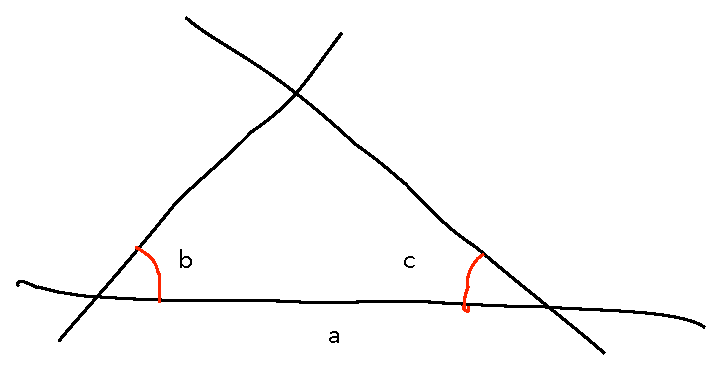
\includegraphics[scale=0.4, angle=180]{media/es-30/triangleACA.eps}
\end{psfrags}
\end{center}
}
\end{minipage}
\begin{tasks}(1)
	\task[c)] Pour terminer la construction du triangle, forme un angle de 30° en partant de l'autre extrémité de ton segment avec ton rapporteur. Les deux demi-droites obtenues par la construction des deux angles doivent se croiser pour fermer le triangle.
\end{tasks}
\vspace{-0.3cm}
%\begin{center}
%\newrgbcolor{ffvvqq}{1 0.3333333333333333 0}
%\psset{xunit=1cm,yunit=1cm,algebraic=true,dimen=middle,dotstyle=o,dotsize=5pt 0,linewidth=2pt,arrowsize=3pt 2,arrowinset=0.25}
%\begin{pspicture*}(-4.3,-0.22)(8.76,6.6)
%\psline[linewidth=2pt](-1.24,1.9)(4.620364913357912,0.6130955426747828)
%\pscustom[linewidth=2pt,linecolor=ffvvqq]{
%\parametricplot{-0.21616358246878076}{0.656501043528384}{0.6*cos(t)+-1.24|0.6*sin(t)+1.9}
%\lineto(-1.24,1.9)\closepath}
%\psline[linewidth=2pt](-1.24,1.9)(3.512795962907222,5.56209373650823)
%\pscustom[linewidth=2pt,linecolor=ffvvqq]{
%\parametricplot{2.4018302955227138}{2.9254290711210125}{0.6*cos(t)+4.620364913357912|0.6*sin(t)+0.6130955426747828}
%\lineto(4.620364913357912,0.6130955426747828)\closepath}
%\psline[linewidth=2pt](4.620364913357912,0.6130955426747828)(0.18859225160557802,4.6577699516408035)
%\begin{scriptsize}
%\psdots[dotstyle=x,linecolor=blue](-1.24,1.9)
%\psdots[dotstyle=x,linecolor=blue](4.620364913357912,0.6130955426747828)
%\rput[bl](-0.32,1.94){\ffvvqq{$50\textrm{\degre}$}}
%\rput[bl](3.42,0.98){\ffvvqq{$30\textrm{\degre}$}}
%\end{scriptsize}
%\end{pspicture*}
%\end{center}
}{1}
\end{resolu}

\begin{exo}{
		\begin{minipage}[t]{0.6\textwidth}{
\vspace{0pt}
Construis en vraie grandeur un triangle $ABC$ dont on connaît un côté $AB$ et les deux angles adjacents $\widehat{BAC}$ et $\widehat{ABC}$. Les valeurs données sont les suivantes : $AB = \tunit{5}{cm}$, $\widehat{BAC} = 40^\circ$ et $ \widehat{ABC} = 60^\circ$. Ci-dessous, tu trouveras un croquis pour t'aider.}
\end{minipage}
\begin{minipage}[t]{0.4\textwidth}{
\vspace{0pt}
\begin{center}
\begin{pspicture}(0,0)(6,4)
    \psdots[dotstyle=x](1,1)(5,1)(3.5,3)
    \pspolygon(1,1)(5,1)(3.5,3)
    \uput[-135](1,1){$A$}
    \uput[-45](5,1){$B$}
    \uput[90](3.5,3){$C$}
    \pcline[linestyle=none,offset=-12pt](1,1)(5,1)\ncput{\tunit{5}{cm}}
    \psarc(1,1){0.8}{0}{40}
    \uput{0.8cm}[20](1,1){$40^\circ$}
    \psarc(5,1){0.8}{126}{180}
    \uput{0.8cm}[160](5,1){$60^\circ$}
\end{pspicture}
\end{center}
}
\end{minipage}}{1}
\end{exo}

\begin{exo}{
		\begin{minipage}[t]{0.6\textwidth}{
		\vspace{0pt}
		Construis en vraie grandeur un triangle $ABC$ dont on connaît un côté $AB$ et les deux angles adjacents $\widehat{BAC}$ et $\widehat{ABC}$. Les valeurs données sont les suivantes : $AB = \tunit{8}{cm}$, $\widehat{BAC} = 50^\circ$ et $ \widehat{ABC} = 70^\circ$. Ci-dessous, tu trouveras un croquis pour t'aider.
		}
		\end{minipage}
		\begin{minipage}[t]{0.4\textwidth}{
		\vspace{0pt}
\begin{center}
\begin{pspicture}(0,0)(6,4)
    \psdots[dotstyle=x](1,1)(5,1)(3.5,3)
    \pspolygon(1,1)(5,1)(3.5,3)
    \uput[-135](1,1){$A$}
    \uput[-45](5,1){$B$}
    \uput[90](3.5,3){$C$}
    \pcline[linestyle=none,offset=-12pt](1,1)(5,1)\ncput{\tunit{8}{cm}}
    \psarc(1,1){0.8}{0}{40}
    \uput{0.8cm}[20](1,1){$50^\circ$}
    \psarc(5,1){0.8}{126}{180}
    \uput{0.8cm}[160](5,1){$70^\circ$}
\end{pspicture}
\end{center}
		}
		\end{minipage}}{1}
\end{exo}

\begin{exo}{
\begin{minipage}[t]{0.6\textwidth}{
\vspace{0pt}
Construis en vraie grandeur un triangle $ABC$ dont on connaît un côté $AC$ et les deux angles adjacents $\widehat{BAC}$ et $\widehat{ACB}$. Les valeurs données sont les suivantes : $AC = \tunit{6}{cm}$, $\widehat{BAC} = 35^\circ$ et $ \widehat{ACB} = 85^\circ$. Ci-dessous, tu trouveras un croquis pour t'aider.}
\end{minipage}
\begin{minipage}[t]{0.4\textwidth}{
\vspace{0pt}
\begin{center}
\begin{pspicture}(0,0)(7,5)
    \psdots[dotstyle=x](1,1)(6,3)(3,4)
    \pspolygon(1,1)(6,3)(3,4)
    \uput[-135](1,1){$A$}
    \uput[-45](6,3){$C$}
    \uput[90](3,4){$B$}
    \psarc(1,1){0.8}{21}{56}
    \uput{0.8cm}[38](1,1){$35^\circ$}
    \psarc(6,3){0.8}{161}{201}
    \uput{0.8cm}[190](6,3){$85^\circ$}
    \psset{shortput=nab,linestyle=none,nrot=:U}
    \pcline(1,1)(6,3)_{\tunit{6}{cm}}
\end{pspicture}
\end{center}
}
\end{minipage}
		}{1}
\end{exo}

\begin{exo}{
\begin{minipage}[t]{0.6\textwidth}{
\vspace{0pt}
Construis en vraie grandeur un triangle $ABC$ dont on connaît un côté $AC$ et les deux angles adjacents $\widehat{BAC}$ et $\widehat{ACB}$. Les valeurs données sont les suivantes : $AC = \tunit{9}{cm}$, $\widehat{BAC} = 125^\circ$ et $ \widehat{ACB} = 65^\circ$. Ci-dessous, tu trouveras un croquis pour t'aider.
}
\end{minipage}
\begin{minipage}[t]{0.4\textwidth}{
\vspace{0pt}
\begin{center}
\begin{pspicture}(0,0)(7,5)
    \psdots[dotstyle=x](1,1)(6,3)(3,4)
    \pspolygon(1,1)(6,3)(3,4)
    \uput[-135](1,1){$A$}
    \uput[-45](6,3){$C$}
    \uput[90](3,4){$B$}
    \psarc(1,1){0.8}{21}{56}
    \uput{0.8cm}[45](1,1){$125^\circ$}
    \psarc(6,3){0.8}{161}{201}
    \uput{0.8cm}[190](6,3){$65^\circ$}
  \psset{shortput=nab,linestyle=none,nrot=:U}
    \pcline(1,1)(6,3)_{\tunit{9}{cm}}
\end{pspicture}
\end{center}
}
\end{minipage}
		}{1}
\end{exo}

\begin{exo}{Construis en vraie grandeur les triangles $ABC$, $DEF$ et $GHI$ dont on connaît un côté et les deux angles adjacents. Les valeurs données sont les suivantes. Pense à faire un croquis avant.
\begin{center}
\begin{tabular}{|c|c|c|c|}
\hline
\textbf{Triangle} & \textbf{Côté connu} & \textbf{Angle 1} & \textbf{Angle 2} \\
\hline
$ABC$ & $AB = \tunit{4}{cm}$ & $\widehat{BAC} = 30^\circ$ & $\widehat{ABC} = 70^\circ$ \\
\hline
$DEF$ & $DE = \tunit{5}{cm}$ & $\widehat{EDF} = 45^\circ$ & $\widehat{DEF} = 60^\circ$ \\
\hline
$GHI$ & $GH = \tunit{6}{cm}$ & $\widehat{HGI} = 50^\circ$ & $\widehat{GHI} = 100^\circ$ \\
\hline
\end{tabular}
\end{center}
}{1}
\end{exo}


\begin{exo}{Construis en vraie grandeur les triangles $ABC$, $DEF$ et $GHI$ dont on connaît un côté et les deux angles adjacents. Les valeurs données sont les suivantes. Pense à faire un croquis avant.
\begin{center}
\begin{tabular}{|c|c|c|c|}
\hline
\textbf{Triangle} & \textbf{Côté connu} & \textbf{Angle 1} & \textbf{Angle 2} \\
\hline
$ABC$ & $AB = \tunit{5,4}{cm}$ & $\widehat{BAC} = 42^\circ$ & $\widehat{ABC} = 73^\circ$ \\
\hline
$DEF$ & $DE = \tunit{4,5}{cm}$ & $\widehat{EDF} = 58^\circ$ & $\widehat{DEF} = 125^\circ$ \\
\hline
$GHI$ & $GH = \tunit{6,3}{cm}$ & $\widehat{HGI} = 62^\circ$ & $\widehat{GHI} = 94^\circ$ \\
\hline
\end{tabular}
\end{center}
}{1}
\end{exo}

\begin{resolu}{Construction d'un triangle 3}{

		\begin{minipage}[t]{0.6\textwidth}{
		\vspace{0pt}
		Construis en vraie grandeur un triangle $ABC$ dont on connaît deux côtés adjacents $AB$ et $AC$ et l'angle $\widehat{BAC}$ formé par ces côtés. Les valeurs données sont les suivantes : $AB = \tunit{5}{cm}$, $AC = \tunit{7}{cm}$ et $\widehat{BAC}=~60^\circ$.
		}
		\end{minipage}
		\begin{minipage}[t]{0.4\textwidth}{
		\vspace{0pt}
\begin{center}
\psset{xunit=0.8cm,yunit=0.8cm,algebraic=true,dimen=middle,dotstyle=x,dotsize=10pt 0,linewidth=1.6pt,arrowsize=3pt 2,arrowinset=0.25}
\begin{pspicture}(0,0)(8,6)
    \psdots[dotstyle=x](1,1)(6,1)(3.5,5)
    \pspolygon(1,1)(6,1)(3.5,5)
    \uput[-135](1,1){$A$}
    \uput[-45](6,1){$B$}
    \uput[90](3.5,5){$C$}
    \psarc(1,1){0.8}{0}{60}
    \uput{0.8cm}[30](1,1){$60^\circ$}
    \psset{shortput=nab,linestyle=none,nrot=:U}
    \pcline(1,1)(6,1)_{$\tunit{5}{cm}$}
    \pcline(1,1)(3.5,5)^{$\tunit{7}{cm}$}
\end{pspicture}
\end{center}

		}
		\end{minipage}

		\vspace{10pt}	

\begin{minipage}[t]{0.6\textwidth}{
\vspace{0pt}
{\bf\blue Programme de construction}
{\blue\begin{tasks}[after-item-skip = 0.3em]
		\task Trace un segment $AB$  de \tunit{5}{cm}.
\task Forme un angle de 50° en partant d'une extrémité $A$ de ton segment en utilisant ton rapporteur. Prolonge suffisamment le trait que tu viens de tracer.
\task Trace un arc de cercle, à l'aide de ton compas, à \tunit{7}{cm} de l'angle que tu viens de construire. L'intersection entre ta demi-droite de l'angle et ton arc de cercle est le sommet $C$ de ton triangle.
\task Pour terminer ta construction, trace le segment $BC.$
\end{tasks}}
}
\end{minipage}
\begin{minipage}[t]{0.4\textwidth}{
\vspace{50pt}
\begin{center}
\newrgbcolor{qqwuqq}{0. 0.39215686274509803 0.}
\psset{xunit=0.8cm,yunit=0.8cm,algebraic=true,dimen=middle,dotstyle=x,dotsize=10pt 0,linewidth=1.6pt,arrowsize=3pt 2,arrowinset=0.25}
\begin{pspicture*}(-1.58,-0.42)(5.36,8.28)
\psline[linewidth=2.8pt,,linecolor=blue](4.,3.)(0.,0.)
\pscustom[linewidth=2.pt,linecolor=qqwuqq]{
\parametricplot{0.6435011087932844}{1.6906986599898821}{0.6*cos(t)+0.|0.6*sin(t)+0.}
\lineto(0.,0.)\closepath}
\psplot[linewidth=2.8pt,,linecolor=blue]{-1.58}{0.}{(-0.--4.964101615137755*x)/-0.5980762113533156}
\parametricplot[linewidth=1.2pt]{1.5992786507582768}{1.7793148984267144}{1.*7.*cos(t)+0.*7.*sin(t)+0.|0.*7.*cos(t)+1.*7.*sin(t)+0.}
\psline[linewidth=2.8pt,,linecolor=blue](-0.8373066958946416,6.949742261192855)(4.,3.)
\begin{scriptsize}
\psdots[dotstyle=x,linecolor=blue](0.,0.)
\rput[bl](0.24,-0.22){\blue{$A$}}
\psdots[dotstyle=x,linecolor=blue](4.,3.)
\rput[bl](4.08,3.2){\blue{$B$}}
\rput[bl](0.,0.94){\qqwuqq{$\alpha = 60\textrm{\degre}$}}
\psdots[dotstyle=x,linecolor=blue](-0.8373066958946416,6.949742261192855)
\rput[bl](-0.76,7.14){\blue{$C$}}
\end{scriptsize}
\end{pspicture*}
\end{center}
}
\end{minipage}

}{1}
\end{resolu}

\newpage
\begin{exo}{
\begin{minipage}[t]{0.6\textwidth}{
\vspace{0pt}
Construis en vraie grandeur un triangle $MNO$ dont on connaît deux côtés adjacents $MN$ et $MO$ et l'angle $\widehat{NMO}$ formé par ces côtés. Les valeurs données sont les suivantes~: $MN = \tunit{4}{cm}$, $MO =\tunit{8}{cm}$ et $\widehat{NMO} = 45^\circ$. Ci-dessous, tu trouveras un croquis pour t'aider.
}
\end{minipage}
\begin{minipage}[t]{0.4\textwidth}{
\vspace{0pt}
\begin{center}
\psset{xunit=0.7cm,yunit=0.7cm,algebraic=true,dimen=middle,dotstyle=x,dotsize=10pt 0,linewidth=1.6pt,arrowsize=3pt 2,arrowinset=0.25}
\begin{pspicture}(0,0)(9,6)
    \psdots[dotstyle=x](1,1)(5,1)(5,5)
    \pspolygon(1,1)(5,1)(5,5)
    \uput[-135](1,1){$M$}
    \uput[-45](5,1){$N$}
    \uput[90](5,5){$O$}
    \psarc(1,1){0.8}{0}{45}
    \uput{0.8cm}[22.5](1,1){$45^\circ$}
    \psset{shortput=nab,linestyle=none,nrot=:U}
    \pcline(1,1)(5,1)_{$\tunit{4}{cm}$}
\pcline(1,1)(5,5)^{$\tunit{8}{cm}$}
\end{pspicture}
\end{center}
}
\end{minipage}
		}{1}
\end{exo}

\begin{exo}{

\begin{minipage}[t]{0.6\textwidth}{
\vspace{0pt}
Construis en vraie grandeur un triangle $PQR$ dont on connaît deux côtés adjacents $PQ$ et $PR$ et l'angle $\widehat{QPR}$ formé par ces côtés. Les valeurs données sont les suivantes : $PQ = \tunit{6}{cm}$, $PR = \tunit{3}{cm}$ et $\widehat{QPR} = 120^\circ$. Ci-dessous, tu trouveras un croquis pour t'aider.

}
\end{minipage}
\begin{minipage}[t]{0.4\textwidth}{
\vspace{0pt}
\begin{center}
\psset{xunit=0.8cm,yunit=0.8cm,algebraic=true,dimen=middle,dotstyle=x,dotsize=10pt 0,linewidth=1.6pt,arrowsize=3pt 2,arrowinset=0.25}
\begin{pspicture}(0,0)(7,4)
    \psdots[dotstyle=x](1,1)(7,1)(4,3)
    \pspolygon(1,1)(7,1)(4,3)
    \uput[-135](1,1){$P$}
    \uput[-45](7,1){$Q$}
    \uput[90](4,3){$R$}
    \psarc(1,1){0.8}{0}{35}
    \uput{0.8cm}[18](1,1){$120^\circ$}
    \psset{shortput=nab,linestyle=none,nrot=:U}
    \pcline(1,1)(7,1)_{$\tunit{6}{cm}$}
    \pcline(1,1)(4,3)^{$\tunit{3}{cm}$}
\end{pspicture}
\end{center}
}
\end{minipage}
}{1}
\end{exo}

\begin{exo}{
		\begin{minipage}[t]{0.6\textwidth}{
		\vspace{0pt}
		Construis en vraie grandeur un triangle $STU$ dont on connaît deux côtés adjacents $ST$ et $SU$ et l'angle $\widehat{TSU}$ formé par ces côtés. Les valeurs données sont les suivantes : $ST = \tunit{7}{cm}$, $SU = \tunit{5}{cm}$ et $\widehat{TSU} = 100^\circ$. Ci-dessous, tu trouveras un croquis pour t'aider.
		}
		\end{minipage}
		\begin{minipage}[t]{0.4\textwidth}{
		\vspace{0pt}
\begin{center}
\psset{xunit=0.8cm,yunit=0.8cm,algebraic=true,dimen=middle,dotstyle=x,dotsize=10pt 0,linewidth=1.6pt,arrowsize=3pt 2,arrowinset=0.25}
\begin{pspicture}(0,0)(8,5)
    \psdots[dotstyle=x](1,1)(8,1)(4,4)
    \pspolygon(1,1)(8,1)(4,4)
    \uput[-135](1,1){$S$}
    \uput[-45](8,1){$T$}
    \uput[90](4,4){$U$}
    \psarc(1,1){0.8}{0}{46}
    \uput{0.8cm}[24](1,1){$100^\circ$}
    \psset{shortput=nab,linestyle=none,nrot=:U}
    \pcline(1,1)(8,1)_{$\tunit{7}{cm}$}
\pcline(1,1)(4,4)^{$\tunit{5}{cm}$}
\end{pspicture}
\end{center}
		}
		\end{minipage}}{1}
\end{exo}

\begin{exo}{Construis en vraie grandeur les triangles $ABC$, $DEF$ et $GHI$ dont on connaît deux côtés adjacents et l'angle formé par ces côtés. Les valeurs données sont les suivantes. Pense à faire un croquis avant.
\begin{center}
\begin{tabular}{|c|c|c|c|}
\hline
\textbf{Triangle} & \textbf{Côté 1} & \textbf{Côté 2} & \textbf{Angle} \\
\hline
$ABC$ & $AB = \tunit{4}{cm}$ & $AC = \tunit{6}{cm}$ & $\widehat{BAC} = 30^\circ$ \\
\hline
$DEF$ & $DE = \tunit{5}{cm}$ & $DF = \tunit{8}{cm}$ & $\widehat{EDF} = 55^\circ$ \\
\hline
$GHI$ & $GH = \tunit{6}{cm}$ & $GI = \tunit{9}{cm}$ & $\widehat{HGI} = 65^\circ$ \\
\hline
\end{tabular}
\end{center}
}{1}
\end{exo}

\begin{exo}{Construis en vraie grandeur les triangles $ABC$, $DEF$ et $GHI$ dont on connaît deux côtés adjacents et l'angle formé par ces côtés. Les valeurs données sont les suivantes. Pense à faire un croquis avant.
\begin{center}
\begin{tabular}{|c|c|c|c|}
\hline
\textbf{Triangle} & \textbf{Côté 1} & \textbf{Côté 2} & \textbf{Angle} \\
\hline
$ABC$ & $AB = \tunit{3,8}{cm}$ & $AC = \tunit{3,8}{cm}$ & $\widehat{BAC} = 35^\circ$ \\
\hline
$DEF$ & $DE = \tunit{5,7}{cm}$ & $DF = \tunit{4,2}{cm}$ & $\widehat{EDF} = 75^\circ$ \\
\hline
$GHI$ & $GH = \tunit{6,3}{cm}$ & $GI = \tunit{8,4}{cm}$ & $\widehat{HGI} = 85^\circ$ \\
\hline
\end{tabular}
\end{center}
}{1}
\end{exo}

\begin{resolu}
{Une dernière construction}
{
	Construis en vraie grandeur un triangle $ABC$ dont on connaît deux côtés adjacents $AB$ et $BC$ et l'angle $\widehat{CAB}.$ Les valeurs données sont les suivantes : $AB = \tunit{7}{cm}$, $BC = \tunit{9}{cm}$ et $\widehat{CAB} = 30^\circ$.

\begin{minipage}[t]{0.5\textwidth}{
\vspace{0pt}
{\bf\blue Programme de construction}
{\blue\begin{tasks}[after-item-skip = 0.2em]
		\task Trace un segment $AB$  de \tunit{7}{cm}.
\task Forme un angle de 30° en partant d'une extrémité $A$ de ton segment en utilisant ton rapporteur. Prolonge suffisamment le trait que tu viens de tracer.
\end{tasks}}
}
\end{minipage}
\begin{minipage}[t]{0.5\textwidth}{
\vspace{0pt}
\begin{center}
\newrgbcolor{ududff}{0.30196078431372547 0.30196078431372547 1.}
\newrgbcolor{qqwuqq}{0. 0.39215686274509803 0.}
\psset{xunit=0.9cm,yunit=0.9cm,algebraic=true,dimen=middle,dotstyle=o,dotsize=5pt 0,linewidth=1.6pt,arrowsize=3pt 2,arrowinset=0.25}
\begin{pspicture*}(-0.58,-1.08)(9,7)
\psline[linewidth=2.4pt,linecolor=blue](-0.24,-0.6)(6.6339021462306444,0.7226750485458379)
\pscustom[linewidth=2.pt,linecolor=qqwuqq]{
\parametricplot{0.19009641940618346}{0.7136951950044822}{0.6*cos(t)+-0.24|0.6*sin(t)+-0.6}
\lineto(-0.24,-0.6)\closepath}
\psplot[linewidth=2.4pt,linecolor=blue]{-0.24}{10.94}{(-2.0752007106288373--4.582421266107833*x)/5.291636357491195}
\psline[linewidth=2.pt,linestyle=dotted,linecolor=blue](2.878804406980365,2.1008045666526947)(6.6339021462306444,0.7226750485458379)
\psline[linewidth=2.pt,linestyle=dotted,linecolor=blue](5.806578619373092,4.636181887930174)(6.6339021462306444,0.7226750485458379)
\parametricplot[linewidth=1.2pt]{1.4794654051211849}{2.9719339971267438}{1.*4.*cos(t)+0.*4.*sin(t)+6.6339021462306444|0.*4.*cos(t)+1.*4.*sin(t)+0.7226750485458379}
\begin{scriptsize}
\psdots[dotstyle=x,linecolor=ududff](-0.24,-0.6)
\rput[bl](-0.36,-0.32){\ududff{$A$}}
\psdots[dotstyle=x,linecolor=blue](6.6339021462306444,0.7226750485458379)
\rput[bl](6.82,0.6){\blue{$B$}}
\rput[bl](0.66,-0.12){\qqwuqq{$\alpha = 30\textrm{\degre}$}}
\psdots[dotstyle=x,linecolor=blue](2.878804406980365,2.1008045666526947)
\rput[bl](2.44,2.12){\blue{$C$}}
\psdots[dotstyle=x,linecolor=blue](5.806578619373092,4.636181887930174)
\rput[bl](5.7,4.94){\blue{$C'$}}
\end{scriptsize}
\end{pspicture*}
\end{center}

}
\end{minipage}
\begin{tasks}[after-item-skip = 0.2em]
	\task[c)] Trace un arc de cercle, à l'aide de ton compas, à \tunit{9}{cm} de $B$. L'intersection entre ta demi-droite de l'angle et ton arc de cercle est le sommet $C$ de ton triangle.
	\task[d)] Tu observes qu'il y a deux réponses possibles, donc un tel triangle existe mais n'est pas unique. 
\end{tasks}
\vspace{-0.5cm}
}{1}
\end{resolu}

\begin{exo}{
\begin{minipage}[t]{0.6\textwidth}{
\vspace{0pt}
Construis en vraie grandeur un triangle $MNP$ dont on connaît deux côtés adjacents $MN$ et $NP$ et l'angle $\widehat{MPN}$. Les valeurs données sont les suivantes : $MN = \tunit{9}{cm}$, $NP = \tunit{5}{cm}$ et $\widehat{NMP} = 50^\circ$. Ci-dessous, tu trouveras un croquis pour t'aider.
}
\end{minipage}
\begin{minipage}[t]{0.4\textwidth}{
\vspace{0pt}
\begin{center}
\begin{pspicture}(0,0)(9,5)
    \psdots[dotstyle=x](1,1)(6,1)(4,4)
    \pspolygon(1,1)(6,1)(4,4)
    \uput[-135](1,1){$M$}
    \uput[-45](6,1){$N$}
    \uput[90](4,4){$P$}
    \psarc(1,1){0.8}{0}{47}
    \uput{0.8cm}[25](1,1){$50^\circ$}
    \psset{shortput=nab,linestyle=none,nrot=:U}
    \pcline(1,1)(6,1)_{\tunit{9}{cm}}
\pcline(4,4)(6,1)^{\tunit{5}{cm}}
\end{pspicture}
\end{center}
}
\end{minipage}
		}{1}
\end{exo}



\exol{ES42}{105}{1}
\exol{ES46}{106}{1}
\exol{ES48}{106}{1}


\end{document}
